%% SW design: klassebeskrivelse devkit Controllers
\newpage

\begin{figure}[htbp] \centering
{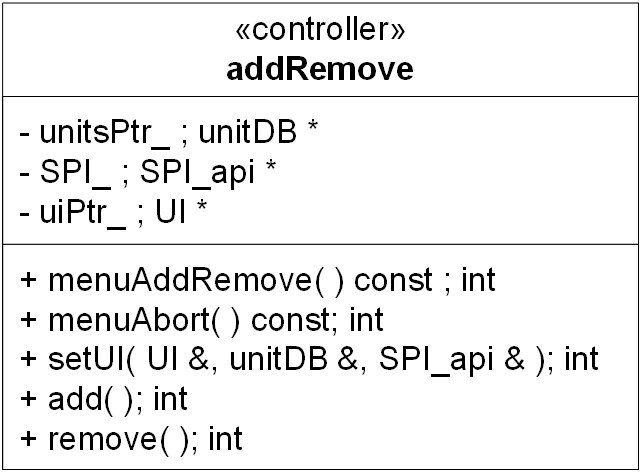
\includegraphics[scale=1.5]{filer/design/Klassediagrammer/sw_addRemove}}
\caption{klassediagram addRemove}
\label{fig:addRemove klassediagram}
\end{figure} 

{\centering
\textbf{addRemove}\par
}
\textbf{Ansvar:} at styre forløbet i UC1: Tilføj / fjern enhed. \

int menuAddRemove( ) const \\
\textbf{Parametre:} Modtager ingen parametre \\
\textbf{Returværdi:} 0 ved succes ellers negativ i overenstemmelse med fejl-listen \\
\textbf{Beskrivelse:} metoden skal styre forløbet i UC1: tilføj fjern.\\

\begin{figure}[htbp] \centering
{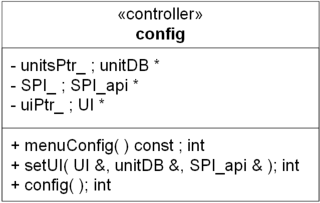
\includegraphics[scale=1.5]{filer/design/Klassediagrammer/sw_config}}
\caption{klassediagram config}
\label{fig:config klassediagram}
\end{figure} 

{\centering
\textbf{Config}\par
}
\textbf{Ansvar:} at styre forløbet i UC2: Konfig. \

int menuConfig( ) const \\
\textbf{Parametre:} Modtager ingen parametre \\
\textbf{Returværdi:} 0 ved succes ellers negativ i overenstemmelse med fejl-listen \\
\textbf{Beskrivelse:} metoden skal styre forløbet i UC1: tilføj fjern.\\

\begin{figure}[htbp] \centering
{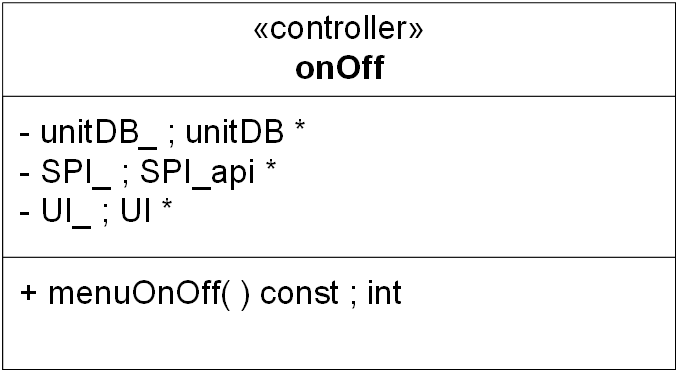
\includegraphics[scale=1.5]{filer/design/Klassediagrammer/sw_onOff}}
\caption{klassediagram onOff}
\label{fig:onOff klassediagram}
\end{figure} 

\newpage

{\centering
\textbf{onOff}\par
}
\textbf{Ansvar:} at styre forløbet i UC3: Aktiver / deajtuver. \

int menuOnOff( ) const \\
\textbf{Parametre:} Modtager ingen parametre \\
\textbf{Returværdi:} 0 ved succes ellers negativ i overenstemmelse med fejl-listen \\
\textbf{Beskrivelse:} metoden skal styre forløbet i UC1: tilføj fjern.\\

\begin{figure}[htbp] \centering
{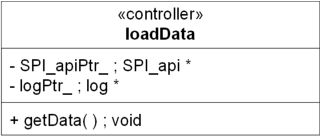
\includegraphics[scale=1.5]{filer/design/Klassediagrammer/sw_loadData}}
\caption{klassediagram loadData}
\label{fig:loadData klassediagram}
\end{figure} 

{\centering
\textbf{loadData}\par
}
\textbf{Ansvar:} at styre forløbet i UC4: Databehandling . \

int menuloadData( ) \\
\textbf{Parametre:} Modtager ingen parametre \\
\textbf{Returværdi:} 0 ved succes ellers negativ i overenstemmelse med fejl-listen \\
\textbf{Beskrivelse:} metoden skal styre forløbet i UC1: tilføj fjern.\\

\begin{figure}[htbp] \centering
{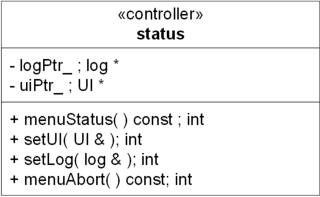
\includegraphics[scale=1.5]{filer/design/Klassediagrammer/sw_status}}
\caption{klassediagram status}
\label{fig:status klassediagram}
\end{figure} 

\newpage

{\centering
\textbf{status}\par
}
\textbf{Ansvar:} at styre forløbet i UC5: Tjek status. \

int menuStatus( ) const \\
\textbf{Parametre:} Modtager ingen parametre \\
\textbf{Returværdi:} 0 ved succes ellers negativ i overenstemmelse med fejl-listen \\
\textbf{Beskrivelse:} metoden skal styre forløbet i UC1: tilføj fjern.\\

\begin{figure}[htbp] \centering
{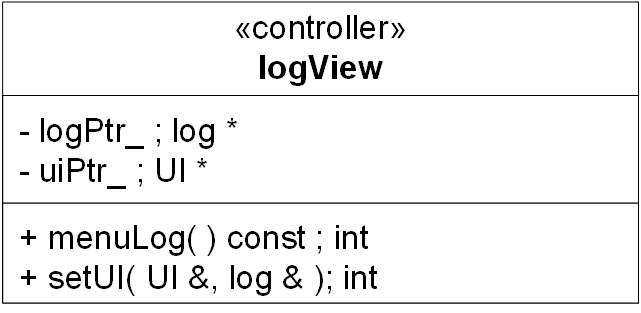
\includegraphics[scale=1.5]{filer/design/Klassediagrammer/sw_logView}}
\caption{klassediagram logView}
\label{fig:logView klassediagram}
\end{figure}

{\centering
\textbf{logView}\par
}
\textbf{Ansvar:} at styre forløbet i UC6: Udskriv log. \

int menuLog( ) const \\
\textbf{Parametre:} Modtager ingen parametre \\
\textbf{Returværdi:} 0 ved succes ellers negativ i overenstemmelse med fejl-listen \\
\textbf{Beskrivelse:} metoden skal styre forløbet i UC1: tilføj fjern.\\

